\subsection{Этапы обработки запроса. Перезапись запросов.}

\subsubsection{Мотивирующий пример}

Пусть имеются следующие таблицы:

\begin{itemize}
	\item \texttt{Students(SId, FirstName, LastName, GId, Year)}.
	      \begin{itemize}
		      \item  Число записей: $10^4$,
		      \item Индексы: \texttt{(SId)} (кластеризованный), \texttt{(Name)};
	      \end{itemize}
	\item \texttt{Groups(GId, Name)}.
	      \begin{itemize}
		      \item  Число записей: $10^3$,
		      \item Индексы: \texttt{(GId)} (кластеризованный), \texttt{(Name)}.
	      \end{itemize}
\end{itemize}

Рассмотрим варианты исполнения следующего запроса:

\begin{lstlisting}[language=SQL]
    select LastName
    from Students natural join Groups
    where Name = 'M34391'
\end{lstlisting}

\begin{itemize}
	\item План 1: наивный подход.
	      \begin{itemize}
		      \item $\pi_{LastName}(\sigma_{Name = M34391}(\sigma_{S.GId = G.GId}(S \times G)))$
		      \item $10^4 \cdot 10^3 + 10^4 \cdot 10^3 + 10^4 + 20 \approx 2 \cdot 10^7$
	      \end{itemize}
	\item План 2: использование алгоритм построения естественного соединения.
	      \begin{itemize}
		      \item $\pi_{LastName}(\sigma_{Name = M34391}(S \bowtie G))$
		      \item $10^4 \cdot 10^3 + 10^4 + 20 \approx 10^7$
	      \end{itemize}
	\item План 3: предварительная фильтрация групп.
	      \begin{itemize}
		      \item $\pi{LastName}(S \bowtie \sigma_{Name = M34391}(G))$
		      \item $10^3 + 10^4 + 20 \approx 10^4$
	      \end{itemize}
	\item План 4: использование индекса \texttt{Students(GId)} (предположим, что он реализован
	      через B-дерево, глубина которого на момент исполнения запроса -- 3).
	      \begin{itemize}
		      \item $\pi{LastName}(S \bowtie \sigma_{Name = M34391}(G))$
		      \item $10^3 + (3 + 20) + 20 \approx 10^3$
	      \end{itemize}
	\item План 4: использование индексов \texttt{Students(GId)} и \texttt{Groups(Name)}
	      (предположим, что последний также реализован через B-дерево, глубина которого на момент
	      исполнения запроса -- 2).
	      \begin{itemize}
		      \item $\pi{LastName}(S \bowtie \sigma_{Name = M34391}(G))$
		      \item $2 + (3 + 20) + 20 \approx 45$
	      \end{itemize}
\end{itemize}

Данный пример показывает, что в зависимости от выбранного плана исполнения запроса разница в
количестве необходимых операций может быть порядковой. В нашем примере -- от $2 \cdot 10^7$
до $45$.

\subsubsection{Обработка запроса}

Этапы обработки запроса:

\begin{enumerate}
	\item Запрос, написанный на SQL, приходит в разборщик запроса, который преобразует его в выражение в
	      реляционной алгебре;
	\item Планировщик запроса планирует, как будет исполняться каждая операция и в каком порядке;
	\item Исполнитель запроса по плану от планировщика исполняет запрос, получая данные из их источника.
\end{enumerate}

Схема этапов изображена на рисунке \ref{query-structure}.

\begin{figure}[H]
	\centering
	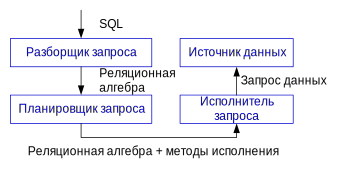
\includegraphics[width=0.8\textwidth]{../assets/kgeorgiy/optimization/Structure_Query.svg.png}
	\caption{Схема обработки запроса}
	\label{query-structure}
\end{figure}

\paragraph{Планировщик запроса}

Планировщик делится на 2 части:

\begin{itemize}
	\item \textbf{Перезапись запроса}. Состоит из набора статических правил оптимизации запроса, не
	      зависящих от конкретного запроса (то есть считающихся полезными всегда);
	\item \textbf{Планировщик}. Выбирает структуру и метод исполнения, а также включает в себя
	      модель оценки, которая дает оценку размеров и распределений результатов запросов. План исполнения
	      перебирается и оптимизируется в зависимости от данных.
	      \begin{itemize}
		      \item \textit{Выбор структуры} -- использование свойств реляционной алгебры,
		            позволяющих преобразовывать запросы так, чтобы результат исполнения был эквивалентным, определение
		            порядка выполнения операций и соединений;
		      \item \textit{Выбор метода исполнения} -- выбор алгоритма исполнения операций.
	      \end{itemize}
\end{itemize}

Схема планировщика запроса изображена на рисунке \ref{query-planner-structure}.

\begin{figure}[H]
	\centering
	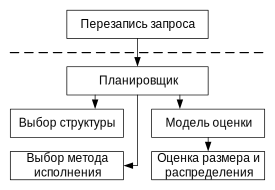
\includegraphics[width=0.8\textwidth]{../assets/kgeorgiy/optimization/Structure_Planner.svg.png}
	\caption{Схема планировщика запроса}
	\label{query-planner-structure}
\end{figure}

Построенные планы оцениваются на сложность с помощью \textbf{модели стоимости}. Каждая операция имеет
стоимость, возможно, зависящую от размеров операндов и ожидаемых результатов. Для оценки
используется статистика по данным и по предыдущим запросам

\subsubsection{Перезапись запроса}

\paragraph{Минимизация набора операций}

\begin{itemize}
	\item \textbf{Преобразование подзапросов}. Использование реляционного исчисления преобразуется
	      в реляционную алгебру, кванторы выносятся.
	\item \textbf{Преобразование соединений}. Внешние соединения устраняются:
	      \begin{align}
		      R_1 \oujoin_{\theta} R_2 & \Rightarrow (R_1 \ljoin_{\theta} R_2) \cup
		      (R_1 \rjoin_{\theta} R_2)                                                   \\
		      R_1 \ljoin_{\theta} R_2  & \Rightarrow \sigma_{\theta}(R_1 \times R_2) \cup
		      (R_1 \setminus \pi_{R_1}(\sigma_{\theta}(R_1 \times \R_2)))                 \\
		      R_1 \rjoin_{\theta} R_2  & \Rightarrow \sigma_{\theta}(R_1 \times R_2) \cup
		      (R_2 \setminus \pi_{R_2}(\sigma_{\theta}(R_1 \times \R_2)))
	      \end{align}
	      Декартово произведение также сводится к естественному соединению. При необходимости одноименные
	      атрибуты переименовываются в одной из таблиц:
	      \begin{align}
		      R_1 \times R_2 & \Rightarrow R_1 \bowtie R_2
	      \end{align}
\end{itemize}

\paragraph{Оптимизация унарных операций}

\begin{itemize}
	\item \textbf{Повторная фильтрация}. Серия из применения фильтраций заменяется на одну
	      фильтрацию с конъюнкцией условий:
	      \begin{align}
		      \sigma_{cond_1}(\sigma_{cond_2}(R)) & \Rightarrow \sigma_{cond_1 \wedge cond_2}(R)
	      \end{align}
	      Порядок проверки условий в конъюнкции на данном этапе не определяется.
	\item \textbf{Повторная проекция}. Серия из применения проекций заменяется на самую внешнюю из
	      них:
	      \begin{align}
		      \pi_A(\pi_B(R)) \Rightarrow \pi_A(R)
	      \end{align}
	\item \textbf{Проекция и фильтрация}. Фильтрация всегда осуществляется до проекции (данное
	      правило позволяет применять предыдущие правила в большем числе случаев):
	      \begin{align}
		      \sigma_{cond}(\pi_A(R)) & \Rightarrow \pi_a(\sigma_{cond}(R))
	      \end{align}
\end{itemize}

\paragraph{Дистрибутивность операций}

\begin{itemize}
	\item \textbf{Фильтрация}. Вынесение фильтрации из множественных операций потенциально
	      уменьшает размер аргументов:
	      \begin{align}
		      \sigma_{cond}(R_1 \cup R_2)      & \Rightarrow \sigma_{cond}(R_1) \cup \sigma_{cond}(R_2) \\
		      \sigma_{cond}(R_1 \cap R_2)      & \Rightarrow \sigma_{cond}(R_1) \cap \sigma_{cond}(R_2) \\
		      \sigma_{cond}(R_1 \setminus R_2) & \Rightarrow \sigma_{cond}(R_1) \setminus
		      \sigma_{cond}(R_2)
	      \end{align}
	      В случае, если условие фильтрации можно разделить на два, каждое из которое проверяет только
	      атрибуты одного из операндов, фильтрацию также можно вынести из естественного соединения:
	      \begin{align}
		      \sigma_{cond_1 \wedge cond_2}(R_1 \bowtie R_2) & \Rightarrow \sigma_{cond_1}(R_1)
		      \bowtie \sigma_{cond_2}(R_2)
	      \end{align}
	\item \textbf{Проекция}. Проекцию можно вынести из объединения:
	      \begin{align}
		      \pi_A(R_1 \cup R_2) \Rightarrow \pi_A(R_1) \cup \pi_A(R_2)
	      \end{align}
	      Однако, этого нельзя сделать при пересечении и разности, поскольку на результат может влиять
	      значение атрибута не из $A$:
	      \begin{align}
		      \pi_A(R_1 \cap R_2)      & \not\Rightarrow \pi_A(R_1) \cap \pi_A(R_2)      \\
		      \pi_A(R_1 \setminus R_2) & \not\Rightarrow \pi_A(R_1) \setminus \pi_A(R_2)
	      \end{align}
	      В случае естественного соединения проекция вносится в каждый аргумент с сохранением атрибутов,
	      необходимых для естественного соединения. Несмотря на то, что число операций увеличивается,
	      распространение проекции может как сокртить размеры аргументов, так и сгруппировать внешние
	      проекции аргументов:
	      \begin{align}
		      \pi_A(R_1 \bowtie R_2) & \Rightarrow \pi_A(\pi_{(A \cup R_2) \cap R_1}(R_1) \bowtie
		      \pi_{(A \cup R_1) \cap R_2}(R_2))
	      \end{align}
\end{itemize}

\paragraph{Коммутативность операций}

Коммутативность позволяет выбрать левый и правый аргумент для несимметричных методов исполнения.
Результаты коммутативных операций равны с точки зрения результата при перестановке аргументов, что
позволяет реализовывать только один вариант перестановки из двух.

\begin{itemize}
	\item \textbf{Коммутативные операции}: $\bowtie$, $\cup$, $\cap$;
	\item \textbf{Некоммутативные операции}: $\setminus$, $\div$, $\gdiv$.
\end{itemize}

\paragraph{Ассоциативность операций}

Ассоциативность позволяет изменять порядок выполнения операций, благодаря чему можно оптимизировать
размеры аргументов.

\begin{itemize}
	\item \textbf{Ассоциативные операции}: $\bowtie$, $\cup$, $\cap$;
	\item \textbf{Неассоциативные операции}: $\setminus$, $\div$, $\gdiv$.
\end{itemize}

\paragraph{Замыкание предикатов}

Из некоторого набора предикатов можно вывести новые правила, которые могут ускорить выполнение
запросов, в частности за счет ``проталкивания'' операции. Некоторые примеры замыкания предикатов:

\begin{align}
	a = b \wedge b = c & \Rightarrow a = b \wedge b = c \wedge a = c \\
	a > b \wedge b = c & \Rightarrow a > b \wedge b = c \wedge a > c \\
	a > b \wedge b > c & \Rightarrow a > b \wedge b > c \wedge a > c
\end{align}

\begin{example}
	\enewline
	\begin{align}
		\sigma_{P_1.p > P_2.p \wedge P_2.p \geq 60}(P_1 \bowtie_{P_1.SId = P_2.SId} P_2)
		\Rightarrow                                       \\
		\sigma_{P_1.p > P_2.p \wedge P_2.p \geq 60 \wedge P_1.p > 60}
		(P_1 \bowtie_{P_1.SId = P_2.SId} P_2) \Rightarrow \\
		\sigma_{P_1.p > P_2.p}(\sigma_{p > 60}(P_1) \bowtie_{P_1.SId = P_2.SId}
		\sigma_{p \geq 60}(P_2))
	\end{align}
\end{example}

\paragraph{КНФ и ДНФ}

Некоторые СУБД преобразуют предикаты в КНФ и ДНФ. Нормальные формы вычисляются слева направо, КНФ
-- до первой лжи, ДНФ --- до первой истины. Это позволяет ускорять запросы, поместив быстро
проверяемые условия как можно левее. Можно также упорядочить условия по строгости, если ее возможно
оценить.

\paragraph{Семантические оптимизации}

Оптимизатор может использовать знания об ограничениях, чтобы заменять запросы на неэквивалентные,
но порождающие те же результаты с учетом ограничений.

\begin{example}
	\enewline
	\begin{align}
		\pi_{LastName}(Students \bowtie Groups) \Rightarrow \pi_{LastName}(Students)
	\end{align}
	Факт, что $Students.GId$ -- внешний ключ, гарантирует, что число студентов не уменьшится, а
	факт, что $Groups.GId$ -- ключ, гарантирует, что число студентов не увеличится. Таким
	образом, преобразование корректно.
\end{example}

\begin{example}
	Введем ограничение: у всех, кто получает стипендию, все оценки не менее 60.

	\begin{lstlisting}[language=SQL]
    check not HasScholarship or 60 <= all
    (select Points from Points where Points.SId = Id)
    \end{lstlisting}

	Рассмотрим запрос, получающий оценки стипендиатов определенной группы по определенному предмету:

	\begin{lstlisting}[language=SQL]
    select Points from Students natural join Points
    where HasScholarship and CId = 10 and GId = M34391
    \end{lstlisting}

	План исполнения, не основанный на ограничениях, выглядит следующим образом:

	\begin{align}
		\sigma_{HasScholarship \wedge CId = 10}(Students \bowtie Points)
	\end{align}

	Воспользуемся ограничением \texttt{HasScholarship}: оценки студентов, имеющих стипендии, не менее
	60.

	\begin{align}
		\sigma_{GId = M34391 \wedge HasScholarship}(Students) \bowtie \sigma_{60 }
	\end{align}
\end{example}

\begin{remark}
	Ограничения, объявленные \texttt{deferrable} и выставленные в \texttt{deferred},
	ограничивают возможности оптимизации, поскольку оптимизатор не может положиться на них. В том числе
	поэтому использование отложенных ограничений может замедлять исполнение запросов.
\end{remark}